\section{Алгоритмы семейства EDA.}

Пусть есть модель, которая является списком вероятностях распределений аллелей для каждого гена. Каждый ген выбирается из своего распределения независимо. Так, для битовых строк модель  будет списком вероятностей выбрать бит-единицу. Будем улучшать модель, а не совокупность выборки. Будем выбирать столько раз из нашей модели и генерировать решение, каков размер выборки, а также высчитывать приспособленность. После чего обновлять модель основываясь на этих решениях и значениях функции приспособленности.

Преимущества:
\begin{itemize}
      \item Простота реализации
      \item Простота теоретических рассуждений
      \item Обновить распределение не сложно
   \end{itemize}

Недостатки:
\begin{itemize}
      \item Обновить распределение не сложно
      \item Нет обучения взаимным зависимостям между генами
      \item Обновить распределение не сложно
      \item Работают не очень хорошо на сепарабельных задачах
   \end{itemize}

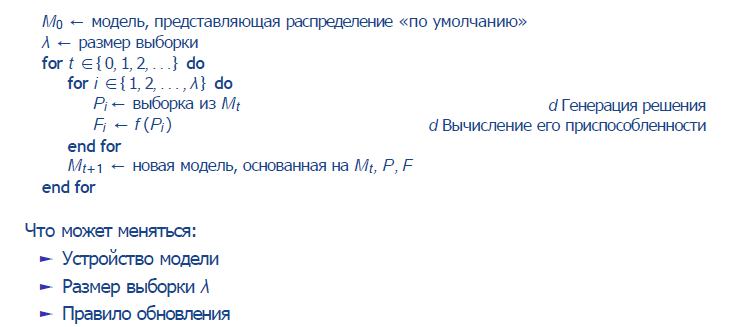
\includegraphics[width=8cm]{images/17bilet.png}  


